\documentclass[en,hazy,blue,noraml,12pt]{elegantnote}
\usepackage{
amsmath,% AMS basic math stuff
amsthm,% AMS theorem defining stuff
amsfonts,% defines the blackboard bold fonts for \Z, \R, etc
}
%证明符号
\usepackage{bbm}
\usepackage[all,cmtip]{xy}
\usepackage{amssymb}
\renewcommand\qedsymbol{$\blacksquare$}



\newcommand{\rr}{\mathbb{R}}
\newcommand{\msp}{(X,\mathcal{E} ,\mu)}
\newcommand{\psp}{(\Omega ,\mathcal{T}   ,P)}
\newcommand{\cc}{\mathbb{C}}
\newcommand{\cha}{\mathbbm{1}}


\title{General Topology
\\ Based on SU MA260
}

\author{X}
\institute{Elegant\LaTeX{} Program}

\begin{document}

\maketitle

\newpage

\tableofcontents

\newpage

%-----------------------------------------------------


\section{Topology Space}\label{def:topological_space}
\subsection{General definition of topology}
\begin{definition}[Topological Space]
    A topological space is a non-empty set \( X \) together with a collection of subsets \(\T \subset P(X)\), satisfying following properties:
    \\1. \(\emptyset\) and \(X\) are in \(\T\).
    \\2. {\bf Satble under finite intersection: }
    for finite sets \(A_n \in \T\), \quad \(\bigcap_n A_n \in \T\)    
    \\3. {\bf Stable under any union:}
    for any sets \(A_i \in \T\),\(i \in I \),\quad \(\bigcup_{i \in I } A_i \in \T\)
\end{definition}

Usually, we denote \( (X,\T)\) to be a topological space, and here \(\T\) is the {\bf topology (structure)} equipped to the space.

\begin{example}[Two trivial topologies on a space]
    Consider a set \( X \). There are two trivial topologies that can be defined on \( X \):
    \begin{itemize}
        \item The \textbf{indiscrete topology} (or trivial topology) on \( X \) is \(\T = \{\emptyset, X\}\).
        \item The \textbf{discrete topology} on \( X \) is \(\T = P(X)\), where \( P(X) \) is the power set of \( X \).
    \end{itemize}
\end{example}

Open and Close are two basic topological concepts, and we give them a definition. Next \(\XT\) will always be a topological space for convienience.

\begin{definition}
    Suppose that A is an subset of the space \(\XT\),
    \begin{itemize}
        \item \(A\) is open if \(A \in \T\).
        \item \(A \) is closed if \(A^c \in \T\), or say \(A^c \) is open.
        \end{itemize}
\end{definition}

Clearly, the property of the open set is just the property of the corresponding topology, and notice tha the closed set is defined to be a duality set of the open set, so we can describle a sapce via the closed set with the same consequence.

\begin{proposition}[The property of the closed set]The definition (\ref{def:topological_space}) is equivalent to the following definition: Suppose \(\mathcal{F}\) is the collection of all closed sets, then \((X,\mathcal{F})\) forms the topological space if it satisfies the following property
    \\1.  \(\emptyset\) and \(X\) are in \(\mathcal{F}\).
    \\2.  Stable under finite unions.
    \\3.  Stabel under any intersections.
\end{proposition}

the proof of the proposition is just the operation between sets, and the third points refers to De Morgan's Law. 

By the three axioms of the topological space, open set can be written by the forms of intersection or union of some open sets. Hence, we choose some open sets and hope that the space can be written by the intersection or union of thses open sets, i.e. we want to choose a basis for a topological space.

\begin{theorem}[Base]$\\$
    Let $\beta$ be a nonempty collection of subsets of a set $X$. If the intersection of any finite number of members of $\beta$ is always in $\beta$, and if $\bigcup \beta = X$, then $\beta$ is a base for a topology \(\T_{\beta}\) on $X$ with the form\\
    \[\T_{\beta} := \{\bigcup_i \beta_i: \beta_i \in \beta \}\]
\end{theorem}

\begin{proof}
    The key point of the proof is \(\emptyset \in \T_{\beta} \), we should clair the notion of the union of sets:
    \[\bigcup_{i \in \emptyset}\beta_i = \emptyset\]
\end{proof}

\begin{example}
    Consider the real line. Let \(\beta\) be the collection of all open interval, then we can verify that \(\beta\) is the base for the common topology of the real line, and we will generalize the result in metric space.
\end{example}


\subsection{Classification of the point in Space}

Whether a set is open or not depends on the elements of the set, and we will call an element in the space "a point" to make it more invisible. firstly, give some vocabulary about the point in the space is given by follwing definition.

\begin{definition}
    suppose \(A \subset X\), \(a \in X\).
    \begin{itemize}
        \item U is a voisinage of \(a\) if U is a open set containing \(a\).
        \item \(a\) is an interior point of \(A\) if there exists a voisinage \(U\) of \(a\) such that \(U \subset A\). 
        \item \(a\) is an accumulation point of \(A\) if \(U \cap A-\{a\} \neq \emptyset \) for any voisinage \(U\) of \(a\).
        \item \(a\) is an adherence point of \(A\) if \(U \cap A \neq \emptyset \) for any voisinage \(U\) of \(a\).
        \item \AA is the set of all interior points of \(A\).
        \item \(A'\) is the set of all accumulation points of \(A\).
        \item $\overline{A}$ is the set of all adherence points of \(A\), or equivalently, $\overline{A} = A \cup A'$, we call it the closure of \(A\).
        \item \(a \) is a isolated point of \(A\) if there exists a voisinage \(U\) of \(a\) such that \(A \cap U-\{a\} = \emptyset\)
    \end{itemize}

    \begin{remark}
        The difference between the accumulation and the adherence points
        always behaves in the isolated point or finite set. Roughly speaking, accumulation points give the possible limits of a sequence in a infinite set if the defined tologycial space is a Hausdorff Space, tha is what the B-W theorem says.
    \end{remark}
\end{definition}

Then we can describe open and closed sets by the different points.

\begin{proposition}
    suppose \(A\) is a subset of \(X\), then
    \begin{itemize}
        \item A is open if and only if \AA = A.
        \item A is closed if and only if \(\overline{A} = A\)
        \item \AA is the biggest open set contained in A.
        \item \(\overline{A}\) is the smallest cloed set containing A.
    \end{itemize}
\end{proposition}

What's more, above definitions can be applied to the union and intersection of different sets, and than some properties can be concluded. It is useful in some basic proof like the properties of the counitious map.

\begin{proposition}
    suppose \(A\) and \(B\) is a subset of \(X\), then
    \\(a) $\overline{A \cup B} = \overline{A} \cup \overline{B}$
    \\(b) $\overline{A \cap B} \subseteq \overline{A} \cap \overline{B}$
    \\(c) $ (A \cup B)^\circ \supseteq A^\circ \cup B^\circ$ 
    \\(d) $ (A \cap B)^\circ = A^\circ \cap B^\circ$
\end{proposition}
 
\subsection{Continous Map}

\begin{definition}
    \(f: X \to Y   \) is a continous map betwwen two topological spaces \(X\) and \(Y\)  if    for any open set \(V\) in \(Y\), the pre-image \(f^{-1}(V)\) is an open set of X.
\end{definition}

\begin{example}[embedding] Suppose that \(Y\) is a subset of topological spaces \(\XT\), we consider the identity map \(\tau: Y \hookrightarrow X \), if we hope the map is a continous map, then the smallest topology defined on \(Y\) is subspace topology \(\mathcal{T}_Y\)

The compostion of functions always happens, the composition fo two continous maps is also a continous map, we omit the proof. Then we give some equvialent statments to understand continuity, it sometimes saves much time when proving.
\end{example}

\begin{theorem}
    If \(X\) and  \(Y\) are tow topological spaces, then the following statements are equvialent:
\\(1) \(f: X \to Y \) is continous.
\\(2) \(\beta\) is a base, any pre-image of the set in \(\beta\) is open.
\\(3) \(f( \overline{A}) \subset \overline{f(A)}\) for any set \(A\) in \(X\).
\\(4) \(\overline{f^{-1}(A)} \subset f^{-1}(\overline{A})\) for any set \(A\) in \(Y\).
\\(5) for any closed set, its pre-image is also closed.

\begin{proof}
    (2) to (3). Just check \(f(A') \subset \overline{f(A)}\). for any accumulation point \(a\) of \(A\), \(f(a) \in Y\), there exists \(B_i \in \beta, i \in I\) such that \(f(a) \in B_i\), so for any open set \(U\) containning, at least some \(B_i \subset U\), so \(f^{-1}(B_i) \cap A-\{a\} \neq \empty \), so \(U-\{f(a)\}\) containing at one point of \(f(A)\).

    (3) to (4). Notice for any \(A \in Y \), \(f^{-1}(A) \in X\), so by (3), we have 
    \[f(\overline{f^{-1}(A)}) \subset \overline{f(f^{-1}(A))} \subset \overline A  \] 
    then add pre-image at both sides we have 
    \[\overline{f^{-1}(A)} \subset f^{-1}(f(\overline{f^{-1}(A)})) \subset f^{-1}(\overline A)\]

    (4) to (5) is trival since \(f^{-1}(A) = \overline{f^{-1}(A)}\) when A is closed. (5) to (1) and (1) to (2) is easy to prove. 
\end{proof}
\end{theorem}

We can construct the product space by continous map.

\begin{definition}[product space]
    We suppose that \((X,\mathcal{T}_X)\) and \((Y, \mathcal{T}_Y)\) are two topological spaces, their cartesian product can be given a topology like below:
    \[\mathcal{T}  = \{U \times V : U \in \mathcal{T}_X, V \in \mathcal{T}_Y\}\]
    Then \((X \times Y, \mathcal{T})\) is a topological space. This construction can be generalized to the n topological spaces.
\end{definition}

The verfiction about the topology is omitted here, the core question here is about \textbf{the universal properties} occuring in the product space. Taking parameterization as an example, we ususally use one parameter to describe a curve in euclidean space, and the latter is actually a catersian set, then ususally the functions can be writted like the form below:
\[ r(t) = (r_1(t), r_2(t) , r_3(t))\]
The component is a simple function. Similarly, we have commuted diagram below about product space:
\[
\xymatrix{
  Z \ar[r]^{f} \ar[d]_{g} \ar@{-->}[dr]& X \\
  Y  & X \times Y \ar[l]_{p_2} \ar[u]^{p_1}
}
\]
where \(p_1\) and \(p_2\) are projections.
\begin{theorem}[Universal property of product space] \label{thm: Universal property of product space} $\\$
    Given three topological space \(X,Y,Z\), suppose \(f\) is a continous map from \(Z\) to \(X\), and \(g\) is a contious map from \(Z\) to \(Y\), and then there exists an unique continous map from \(Z\) to product space \(X \times Y\) such that above diagram commute.

i.e. If \(C(Z,X)\) and \(C(Z,Y)\) are the two sets of all continous maps form \(Z\), then there exist a bijection betwwen \(C(Z,X \times Y)\) and \(C(Z,X) \times C(Z,Y)\) 

\begin{proof}
    We define \(h: Z \to X \times Y, z \mapsto (f(z),g(z))\), then for any open set \(U \times V\) in \(X \times Y\), we have 
    \begin{align*}
        h^{-1}(U \times V) &= \{z \in Z: h(z) = (f(z),g(z)) \in U \times V\} \\
        &= \{z \in Z: f(z) \in U, g(z) \in V\} \\
        &= f^{-1}(U) \cap  g^{-1}(V) 
    \end{align*}
    clearly that it is open since \(f\) and \(g\) are continous, so our definition is well-defined. The leaving problem is uniqueness, we suppose that \(\bar{h}\) is another continous such that diagram commute, then we have \(p_1 \circ \bar{h} = f\) and \(p_2 \circ \bar{h} = g\), so 
    \[\bar{h} (z)= (p_1 \circ \bar{h}(z), p_2 \circ \bar{h}(z)) = h(z)\]
    which means that our definition is unique (Even nautral). 
\end{proof}

\end{theorem}

The exists a similar map between two topological space like isomorphism in group theory or linear algebra, which keeps the topological structure, in fact it is a special continous map.
\begin{definition}
    \(f: X \to Y\) is a \textbf{hoemomorphism} between topological space \(X\) and \(Y\) if f is bijective and continous, and \(f^{-1}\) is also continous. The Two space is hoemomorphic if there exists a hoemomorphism.
\end{definition}


\begin{remark}
    hoemomorphism invites a corresponding between the two topologies, and we give an example to clair that the couniuity of the inverse is necessary: Given a complex-value bijection \(f : [0,1) \to S^1 , x \mapsto e^{2 \pi i x}\), but f is contionous but \(f^{-1}\) is not since \(f([0,1/2)\) is not open in \(S^1\). So \(f\) is not a hoemomorphism.

    What are the "same"(hoemomorphic) spaces? The key problem here is that Whether there exists other potential hoemomorphism. To get the answer we should need to know more about topological property that the hoemomorphism can keep, after we can find that \([0,1/2)\) is not a compact space but \(S^1\) is compact, which means that the two space can not be hoemomorphic.
\end{remark}

\section{Metric Space}

The motivation of metric space is from distance, it is a geometric concept which actually can be seen as a binary operation.
\begin{definition}
    A distance on a non-empty set \(X\) is a postive function
    \[d: X \times X \to \R^+\]
    satisfies three axioms:
    \\\textbf{Definite:} \quad \(d(x,y) = 0 \iff x = y\),
    \\\textbf{Symmetry:} \quad \(d(x,y) = d(y,x)\),
    \\\textbf{Triangular inequality:} \quad \(d(x,y) + d(y,z) \geq d(x,z)\)
\end{definition}

Usually, we call \(\Xd\) is a metric space. A classic distance is euclidean space \(E^n\) with a function which gives the physics distances of two points 
\[d(x,y) = (\sum_{i=1}^{n}|x_i-y_i|^2)^{1/2}\]
Next we will study the corresponding topological propeerties in metric space, but we should keep in mind that metric space is a important type of topological space, by learning that we grasp the abstract concept like open and closed set, anyway, more example is good to find the corresponding connection.

\subsection{Topological structure of metric space}

We firstly prove that metric space is a topology space by finding the base for topology. For a space \(\Xd\), we define the open ball is a set centred on some point with some radius:
\[B_d(x,r) = \{y\in X: d(x,y) < r\}\]
Notice that if \(r = 0\), the open set is empty. Then we can find that the collection of all open sets is a base for the space. To find that we fix
\(a \in X\), then \(\cup_{n \in \n} B(a,n) = X\) since for any \(x \in X\), \( d(x,y) \in [k,k+1) \) for some entier \(k\) by the properties of real line, clearly that \(x\) is in a open ball. The core problem here is to verify the stability of the finite intersection of the base.

If the intersection of two open sets is not empty, then we let \(y \in B(x,r) \cap B(x',r')\). In \(B(x,r)\) there exists \(\delta\) such that \(B(y,\delta) \subset B(x,r)\), see the figure below.
\begin{figure}[h]
    \centering
    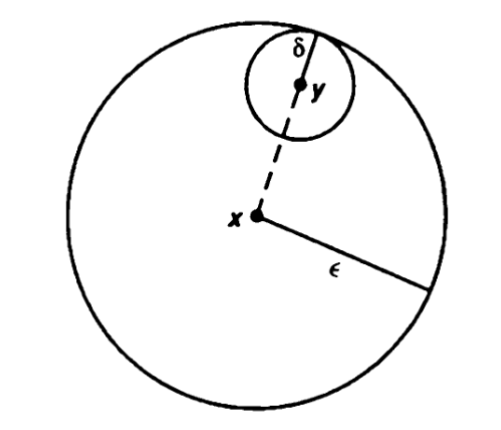
\includegraphics[width=0.4\textwidth]{fig/1.png}
\end{figure}
Similarly, there exists \(\delta'\) such that \(B(y,\delta') \subset B(x',r')\), hence we take \(\xi = min(\delta,\delta')\) to make \(B(y,\xi) \subset B(x,r) \cap B(x',r')\), finally we can find that the intersection can be written by the infinite union of open sets:
\[B(x,r)\cap B(x',r') = \cup_{y \in B(x,r)\cap B(x',r')} B(y,\xi_y)\]

All open ball gives a topology of the metric space, then clearly any open ball is a open set, and if we see the open all as a basic elemnts of open sets then we can rewrite the \textbf{interior} here:

" \(x\) is a interior of the set \(A\) if there exists a positive \(r>0\) such that \(B(x,r) \subset A\)."

Notice the definition we got is not direct, we firstly get an open ball containing \(x\) which is a subset of \(A\), then choose an open ball centering at \(x\), the technic here is simalar with the construction in the figure above.
According to this we can get the natrual definition of the open set in mertic space as following:

\begin{definition}
    \(A\) is an open set in metric space \(\Xd\) if for any \(x \in A\), \(\exists r>0\) such that \(B_d(x,r) \subset A\).
\end{definition}

By same thought, the other definition of points can be rewritten here just by replacing the voisinage with the open ball centering at the point itself.

\begin{definition}
    \(A\) is a closed set in metric space if for any \(x \in A\), any \(r>0\), we have \(B(x,r) \cap A \neq \emptyset\).
\end{definition}

We should notice that the definition here is all natural if we have know just a little thing about point-set topology, and the proof about the properties like closure and interior set are all same just change open ball to be voisinage. Although topology is more general, always remmeber that the motivation of the definition in general topology is from the special things in metric space even \(\R\).

Finally we give the corresponding definition of continous map, it refers to the famous motivation of the pint-set topology
\begin{theorem}[Continuity]
    \(f:X \to Y\) is continous if and only if for all \(a,b \in X\), we have
    \[\forall \epsilon>0, \exists \delta>0 s.t. \quad d_X(a,b)<\delta \Rightarrow d_Y(f(a),f(b )) <\epsilon\]

    \begin{proof}
        
    \end{proof}
\end{theorem}
\subsection{Sequential Caracteristics}
One thing that we may not know is that metric space is indeed a Hausdorff space, but it does not matter, One key thing here is that we should care about the sequential properties in metric space and we can define the convergence of the sequence.
\begin{definition}
    suppose \(\xn\) is a seuqence of the metric space \(\Xd\), then it converges to some point \(a \in X\) if 
    \[\forall \epsilon > 0 , \exists N \in \n, s.t. \quad n \geq N \Rightarrow d(x_n,a) < \epsilon\]
\end{definition}


By the definition, We firstly prove a key property of closed set here.

\begin{proposition}[Sequential caracteristics of closed sets] $\\$
    A set is closed in a metric space if and only if for any convergent sequence of the set, the limit is also in the set.

    \begin{proof}
        
    \end{proof}
\end{proposition}

\begin{example}
    We consider the set of hyperbole \(H = \{(x,y) \in \R^2 : xy=1\}\).
    \\1. Suppose \((x_n,y_n) \in H\) forms a sequence converges to \((a,b) \in \R^2\).
    \\2. \(x_ny_n =1\) for any entier \(n\).
    \\3. \(ab = \lim x_n \lim y_n = \lim x_ny_n = 1\), so \((a,b) \in H\), i.e. \(H\) is closed.
    \\ I give the detail of the verfiction here is to check that what the caracteristics depends on. Step 1 and 2 is just the translation of the given condition, so we just check step 3 and then we can find that step 3 depends on \textbf{the properties of the limit in real line} (the product of the limit), and that is the response here.

    The definition of the convergence can be extended to the function.
    \begin{definition}
        Suppose \(f: X \to Y\) is a function between two metric space, then \(f(x)\) converges to \(L \in Y\) at point a if 
        \[\forall \epsilon > 0, \exists \delta >0, s.t. \quad 0<d_X(x,a)<\delta \Rightarrow d_Y(f(x),L)< \epsilon \]
        We write is as \(\lim_{x \rightarrow a}f(x) = L\)
    \end{definition}
    The definition can be modified to be well-defined if the limit is inifinit, but we should pay attention that limit is a local tendency, that means the distrubution aroud the point determines the limit of the function. For example, let us consider a real function
    \[f(x) = \begin{cases}
        x, \quad x\neq 0 \\
        2, \quad x=0
    \end{cases}\]
    We can verify that \(f\) converges to 0 when \(x\) tends to zero, not \(f(0) =2\), that means in general
    \[\lim_{x \rightarrow a} f(x) \neq f(a) = f(\lim_{x \rightarrow a} x)\]

    Another problem is about \textbf{islated point}, we can not define the limit at the isolated point, we also consider a real function
    \[f(x) = \begin{cases}
        x, \quad x\in [0,1] \\
        2, \quad x=2
    \end{cases}\]
    Clearly that the function is defined on \([0,1]\cup \{2\}\), but the limit at 2 dose not exist though the function can be given a good extension \(x \mapsto x\), where the limit at 2 is 2. So when we consider the convergence of the function, the defined set is restricted to be the set of the accumulation points to avoid the above inconsistency. However the definition of the continous map ensures that the conuity at the islated point, so it makes sense to consider the all adherence of a defined set.
\end{example}

\begin{proposition}[Sequential caracteristics of the continuity] $\\$
    Suppose \(f : X \to Y\) is a continous map, then for a sequecne \(\xn\) of \(X\) which converges to \(x \in X\), the sequence \((f(x_n))_{n \in \n}\) of \(Y\) converges to \(f(x)\), i.e.
    \[\lim_{n \rightarrow \infty} f(x_n) = f(\lim_{n \rightarrow \infty} x_n) \]
    
    \begin{proof}
        Let \(d_Y(f(x),f(x_n))<\epsilon\), the continuity of \(f\) implies
        \[d_X(x,x_n) < \delta\]
        for some \(\delta >0\), and then the convergence of the sequence implies a entier \(N\) such that \(n \geq N \) implies \(d_Y(f(x),f(x_n))<\epsilon\).
    \end{proof}

\end{proposition}

Another sequential caracteristics of the metric space is comapctness, we wil later give an equivalent proposition about compact set, which is motivated from \textbf{Bolzano-Weierstrass Theorem}: all the bounded sequence in real line have a convergent subsequence.

To end this part we give a imortant propoistion in functional analysis.

\begin{proposition}\label{CB closed in B}

    \(X\) and \(Y\) are two metric space and let \(CB(X,Y)\) be the set of all bounded continous functions from \(X\)  to \(Y\), and \(B(X,Y)\) be the set of all bouded functions from \(X\) to \(Y\), then \(CB(X,Y)\) is a closed set of \(B(X,Y)\) equipped with the supremum metric \(d_{\infty}\):
    \[d_{\infty}(f,g) = \sup_{x \in X} d_Y(f(x),g(x))\]

    \begin{proof}
        Suppose \((f_n)_{n \in \n}\) is a sequence of \(CB(X,Y)\) which converges to some bounded fonction \(f\), then for any \(a \in X\),
        \[d_Y(f_n(a),f(a)) \leq d_{\infty}(f_n,f)<\epsilon\]
        The uniform convergence of \(\fn\) gives a entier \(N\) such that 
        \[n \geq N \Rightarrow d_Y(f_n(a),f(a))<\epsilon\]
        which means that the seuqence \((f_n(a))_{n \in \n}\) of \(Y\) converges to \(f(a)\). Then we can prove the conuity of \(f\) by the inequality
        \[d_Y(f(x),f(a)) \leq d_Y(f(x),f_n(x))+d_Y(f_n(x),f_n(a))+d_Y(f_n(a),f(a))\]
        the second term can implies an entier since each \(f_n\) is continous, so we finish the proof.
    \end{proof}
\end{proposition}

\subsection{Comparison of the distance}

The product space in metric space can have many possible distances. Suppose \(X\) and \(Y\) are two metric space there exists three common distance defined to their product \(X \times Y\):
\begin{itemize}
    \item \(L^1\) metric: \(d_1 ((x,y),(x',y')) = d_X(x,x') + d_Y(y,y')\)
    \item \(L^2\) metric: \(d_2 ((x,y),(x',y')) = \sqrt{d_X^2(x,x')+d_Y^2(y,y')}\)
    \item $L^\infty$ metric: \(d_{\infty} ((x,y),(x',y')) = \max \{d_X(x,x'),d_Y(y,y')\}\)
\end{itemize}

By comparing the distance we can get much information, for example, the continuity of a identity map can not be ensured when we want to change a metric for the same space.

\begin{proposition}
    Suppose \(d\) and \(\tau\) are two different distances for the space \(X\), then the identity map from \(\Xd\) to \((X,\tau)\) is continous if and only if there exists an positives \(c\) such that \(\tau \leq cd\).

    \begin{proof}
         for any \(x,x'\in X\), we have 
        \[\tau(id(x),id(x')) \leq c d(x,x')\]
        We take \(\delta < \epsilon/c\), then it is clair.
    \end{proof}
\end{proposition}

According to the proposition, we can easily find that the identity map between the three space sharing same sets with three different distances are hoemomorphisms, just by inequality
\[d_{\infty} \leq  d_2 \leq d_1 \leq 2d_{\infty}\]
Which means that three spaces have the same open set, or they are "same" topological space. We can conculde the comparison by a equavlence relation.

\begin{definition}
      Suppose \(d\) and \(d'\) are two distances for the space \(X\), then we call the two distances are \textbf{equivalent distance} if there exists two positives \(m,M\) such that 
        \[md' \leq d \leq Md'\]
\end{definition}

So clearly, we can have the following theroem
\begin{theorem}[Equivalent distance implies the same topology] $\\$
    If \(d\) and \(d'\) are two equiavlent distances for the space \(X\), then their topology defined by the open ball is same. 
    \\(or we can say)If \(\beta\) and \(\beta '\) are two topology base for \(X\) invited by two metrics, then the they are two base for the same topology.
\end{theorem}

Goemetrically, a unit open ball (radius is 1) under a metric may be not a "ball", for example in space \(\R^2\) with \(L^{\infty}\) metric, the open ball \(B(a,1)\) is a square centred at a with sides length 2, it is a open cube actually. Generally, it seems that whatever figure the open ball is, it can be approximated by the infinite union of real "balls", but it works only in a space whic can be imaged like plane, i.e. the vector space with finite dimension. In conclusion, whatever the figure we define the open ball is, it always gives the same topology in finite dimensional vector space, we will later conculde the result.  

\subsection{Normed Vector Space}
We now introduce an important metric space. Usually, it appears togetehr with an inner product space, and it is very useful for us to study the properties of the function.
\begin{definition}
    Given a vector space \(E\) over a field \(\K\), we call it a \textbf{normed (vector) space} if the space is equipped with a norm \(N: E \to \R^+\) satisfying three axioms
    \\\textbf{Definiteness}: \(N(x) = 0 \iff x=0 \)
    \\\textbf{Homogeneity:} \(N(\mu x ) = |\mu|N(x)\) pour any \(\mu \in \K\)
    \\\textbf{Triangualr Inequality:} \( N(x+y) \leq N(x) + N(y)\)
\end{definition}

Clearly here the norm invites a metric to \(E\) by 
\[d(x,y) = N(x-y)\]
The Symmetry axiom is ensured by the commutative addition of the vector space. It is important since inner poroduct implies the norm, and inner product is an improtant operation occruing in many places. Another reason is that in metric space we give the definition of the "distance" but we do not give the definition of "length", although the length seems can be seen as the distannce of two endpoints if we consider a stright line. However the distance determines how to measure the length of the line with two endpoints, but whether the line is stright or not depends on the metric.

\begin{example}[Metric does not implies norm] $\\$
    We consider a metric \(d(x,y) = 1 \) if \(x \neq y\). 
\end{example}
The open ball and closed ball here can be wirtten by the form 
\[B(x,r) = \{y \in E : N(x-y) < r\}\]
\[B_F(x,r) = \{y \in E : N(x-y) \leq r\}\]
One of the most important characteristics is that the open ball here is \textbf{convex} (The statement is not true in general metric space), which implies that the closrue of the open ball is exactly a cloesd ball:
\[\overline{B(x,r)}  = B_F(x,r)\]
This equality is not true in general metric space. The detail of the proof can be found in TD1 and TD4.









\section{Complet Space}
\subsection{Basic properties}
We have known that we can talk sequence in metric space, so some space described by sequence can be montioned here.

\begin{definition} $\ $
    \begin{itemize}
        \item A sequence\(\xn\) is a \textbf{Cauchy sequence} of the metric space \(\Xd\) if 
        \[\forall \epsilon >0, \exists N \in \n, s.t. \quad n,m\geq N \Rightarrow d(x_n,x_m) < \epsilon \]
        \item A metric space is \textbf{complet} if all Cauchy sequence in it is convergent.
    \end{itemize}
\end{definition}

\begin{remark}
    It is easy to prove the two properties about Cauchy sequence
    \begin{itemize}
        \item Convergent sequecne implies Cauchy sequence.
        \item Cauchy Sequence implies bounded space.
    \end{itemize}
    \(\R\) is a typical complet space with common metric in camparison with \(\mathbb{Q}\), a classic seuqence of rational number converging to a irrational number is a series \textbf{(Basel's problem)}
    \[1 + \frac{1}{2^2}+\frac{1}{3^2}+ \dots = \frac{\pi^2}{6}\]
    It is easy to prove that the sequence is Cauchy in \(\mathbb{Q}\) but not convergent. There are several types of divergence, the problem here is that we can not find a sepcial point to which the sequence converges though we know it tends to something, the defect is in the space or not the sequence itself! Hence "completness" is a suitbale analogies.
\end{remark}

    One space may not be complet if we change the metric, we take \(\R\) as a example, and define a metric \(d(x,y) = |e^x-e^y|\), we can prove that it is not complet. Taking a Cauchy sequence \(\xn\),then 
    \begin{align*}
        x_n \rightarrow_{n\rightarrow \infty} x & \iff e^{x_n} \rightarrow_{n \rightarrow \infty} e^x 
    \end{align*}
    We know that the sequence \((-n)_{n \in \n}\) is not Cauchy  under the common metric, but it is a Cauchy sequence under the defined metric above. A fact we should notice that two metric gives the same topology, but it can not guarantee the completness, but we can give a suffisant condition.

    Finally we can just see \(\R\) as the completness of \(\q\) with its common absolutely value, formally it refers to a equiavlent realtion on the set of all Caucht sequence in \(\q\) by 
    \[(\xn) \sim (\yn) \iff (x_n-y_n)_{n \in \n} \rightarrow_{n\rightarrow \infty} 0\]
    \begin{proposition}[Equivalent distance implies co-complet] $\\$ \label{Equivalent distance implies co-complet}
        If a spcae \(X\) have two equivalent distance \(d\) and \(d'\), then \(\Xd\) is complet if and only if \((X,d')\) is complet.

        \begin{proof}
            Just two steps. Firtstly, a seuqence is a Cauchy sequence in \(\Xd\) if and only if it is a Cauchy sequence in \((X,d')\), then prove that if in two space a same cauchy sequence will have the same limit. The proof is finished by the inequality of the equivalent distance.
        \end{proof}
    \end{proposition}

    An immediate result can be given considering \(\R^n\)
    \begin{corollary}
        \(\R\) equipped by one of three common metrics(\(L^1,L^2,L^{\infty}\)) is always a complet space.
    \end{corollary}

\subsection{Induced complet space}

Here we will consider several natural complet space by cartesian product or restriction, which is all common technic.

\begin{proposition}[The completness of the product space]$\\$ \label{complet product space}
    Given two complet spaces \(\Xd\) and \((Y,d')\), their product \( X \times Y\) is complet if the equipped metric is \(L^{\infty}\) metric 
    \[d_{\infty} = \max (d,d') \]

    \begin{proof}
        Assume that \(((x_n,y_n))_{n \in \n}\) is a cauchy sequence of the product space, by the given metric we can conclude that \(\xn\) and \(\yn\) are the cauchy sequence of \(\Xd\) and \((Y,d')\) respectively, so there exist \(x \in X\) and \(y \in Y\) such that the two sequences converge. Finally we just need to verify that the sequence \(((x_n,y_n))_{n \in \n}\) converges to \((x,y)\).
    \end{proof}
\end{proposition}

\begin{corollary}
    \((\R^n, d_{\infty})\) is a complet space with \(L^\infty\) norm, and then again by ~\ref{Equivalent distance implies co-complet} we have that \(\R^n\) is a complet space with one of three common metrics.
\end{corollary}

\begin{proposition}[Completness of subspace]$\\$
    Given \(\Xd\) is a complet metric space, a subspace \(Y \subset X\) is complet if and only if \(Y\) is \textbf{closed} in \(X\).

    \begin{proof}
        
    \end{proof}
\end{proposition}


One interesting example is a function space, which we will always use it latter, notice that \(B(X,Y)\) is a metric space with the \(L^{\infty}\) metric, and \(CB(X,Y)\) is a induced subspace, together with the result ~\ref{CB closed in B} we can immediate get that \(CB(X,Y)\) is complet if \(B(X,Y)\) is complet, so let us investigate when it is complet.

Notice that for any \(x \in X\), we have the following inequality
\begin{equation}
    d_Y(f_n(x),f_m(x)) \leq d_{\infty}(f_n,f_m) 
    \label{eq:1}
\end{equation}
clearly that we hope \(Y\) is a complet space which implies a sequence in \(Y\) for any \(x\), and then it defines a function that a given cauchy sequence converes to.
 
\begin{proposition} \label{BXY complet if Y complet}
    \((B(X,Y),d_{\infty})\) is complet if \((Y,d_Y)\) is complet.

    \begin{proof}
        Suppose that \(\fn\) is a Cauchy sequence in \(B(X,Y)\), and we fix a value \(a \in X\) and then \((f_n(a))_{n \in \n}\) is a Cauchy sequence by (\ref{eq:1}), and it is convergent since \(Y\) is complet. So we define a function \(f(x) = \lim_{n \rightarrow \infty}f_n(x)\), and then for any \(a,b \in X\), we have 
        \[d_Y(f(a),f(b)) \leq d_Y(f(a),f_N(a))+d_Y(f_N(a),f_N(b))+ d_Y(f(b),f_N(b))\]
        which implies that \(f\) is bounded, so \(f \in B(X,Y)\). Finally we will prove that \(\fn\) converges to \(f\). just let \(m\) in (\ref{eq:1}) tends to \(\infty \) and then we get for any \(x \in X\)
        \[d_Y(f_n(x),f(x)) \leq \epsilon\]
        and then we can get the expected result.
    \end{proof}
\end{proposition}

\subsection{Fixed point Theorem}
One strong and useful result in complet space is about fixed point, it always appears in a reccurence like 
\begin{equation}
    \begin{cases} \label{eq:fixed point seq}
    x_0 = x \\
    x_{n+1} = f(x_n)
\end{cases}
\end{equation}

We will firstly prove the corresponding theorem, and then we will see how it works in the theory of differential equations.

\begin{theorem}[Banach-Picard fixed point theorem]$\\$
    Given a metric space \(\Xd\), and a fonction \(f: X \to X\) is contract if there exists a positive \(k < 1\) such that \(d(f(x),f(y))\leq kd(x,y)\) for any \(x,y \in X\).

    If the space is complet and a function is contract, then the function has an unique fixed point \(x=a\) (such that \(f(x) = x\)), and we have 
    \begin{itemize}
        \item for any \(x \in X\), the sequence \((f^n(x))_{n \in \n}\) of \(X\) converges to \(a\).
        \item for any \(x \in X\), \(d(x,a) \leq \frac{1}{1-k} d(x,f(x))\)
    \end{itemize}
    
    \begin{proof}
        Firtstly we will show the existence of the fixed point. Just use the sequence defined in (\ref{eq:fixed point seq}), the sequence is cauchy because
        \begin{align*}
            d(x_{n+1},x_n) &= d(f(x_n),f(x_{n-1})) \\
            &\leq k \cdot d(x_n,x_{n-1}) \\
            &... \\
            &k^n \cdot d(x_1,x_0)
        \end{align*}
        So \(\xn\) converges to some \(a \in X\) since the given space is complet. And easily to prove that a contract function is continous, then we can find 
        \[a = \lim x_{n+1} = \lim f(x_n) = f(\lim x_n) = f(a)\]
        The fixed point is unique. Suppose that there exists another different fixed point \(a'\), then we have two following corollaries:
        \[d(a,a') \leq d(f(a), f(a')) \leq k d(a,a')\]
        which implies \(k \geq 1\), it is absurd since \(f\) must be contract. 

        We finish the main part of proof, and the first collary is an immediate result from the main part, we just prove the second corollary. 
        \begin{align*}
            d(f^n(x),x) &\leq d(f^n(x),f^{n-1}(x)) +...+ d(f(x),x) \\ 
            & \leq (k^{n-1}+...+k+1)d(f(x),x) \\
            &= \frac{1-k^n}{1-k}d(f(x),x)
        \end{align*}
        Just take the limit of both sides we can get the expected result.
        \end{proof}
\end{theorem}

Now we will turn our attention to see how the theorem works in differential equations. In 18th century, mathematicens are familiar with the solutions of the different ordianary differential equations, but how to give a general conculusion about the uniqueness of the solution of a Cauchy problem (I-C problem)?

\begin{example}
    We consider the following cauchy problem 
    \[\begin{cases}
        f'=f \\
        f(0)=1
    \end{cases}\]
    By the fundamental theorem of calculus we can know that the problem has soulution if and only if for any \(x\), there exists a continous function such that 
    \[f(x) = 1+ \int^x_0 f(t)dt\]
    We consider a opreator which maps a function to a new function, so the above condition can be transformed to the existence of the fixed point of a operator \(T: CB((-a,a),\R) \to CB((-a,a),\R)\) defined by 
    \[T(f) = 1+\int_0^{.}f(t)d(t)\]
    we can verify that the opreator is contract if we choose \(a =1/2\):
    \begin{align*}
        d_{\infty}(T(f),T(g)) &= \sup_{x \in (-a,a)}|\int_{0}^{x}f(t)-g(t)dt| \\
        &\leq a \cdot d_{\infty}(f,g)
    \end{align*}
    \(CB((-a,a),\R)\) is complet according to the previous disccusion, so we can conculde that there exists an unique opreator in \(CB((-a,a),\R)\) such that \(T(f)=f\), which implies that the solution of the Cauchy problem here is unqiue in interval \((-a,a)\). 

    An question is that whether the soultion is unique in whole \(\R\)? It is no diffcult to extend the function with the same technic. 
\end{example}

\subsection{Banach Space}

A complet normed vector space is a \textbf{Banach Space}. It is just a  definition to classify a special space, special naming is often accompanied by profound properties about a certain object. 

A classic Banach space is a functional space, we give below.

\begin{proposition}
    \((\mathcal{C} [0,1],\|\cdot\|_{\infty})\) is a Banach space.

    \begin{proof}
        The complet of the space is directly from the general proposition \ref{BXY complet if Y complet}, notoce here \(f \in \mathcal{C} [0,1]\) means the continous function from \([0,1]\) to \(\R\). And we should prove that the space is a vector space, that is direct from the algebra properties of the continuity, that is a good exercise for both analysis and linear algebra.
    \end{proof}
\end{proposition}

We notice that the convergence of the sequence in Banach space depends on the \(\R\), so we generalize the concept of the series here.
\begin{definition}[Series] 
    Given a normed space \((E,\|\cdot\|)\), a series is the infinite sum of a sequence in the space, usually we denote it \(\sum u_n\). a series \(\sum_{n \in \n}u_n\) is convergent (to \(L\)) if a corresponding sequence(paritial sum) \(S_n= \sum_{k=0}^{\infty}u_n\) is convergent (to \(L\)).

    A series \(\sum_{n \in \n}u_n\) is \textbf{absolutely convergent (normal convergent)} if the series \(\sum_{n \in \n}\|u_n\|\) is convergent in \(\R\).
    
\end{definition}

Then some classic results about the series can be proved

\begin{proposition}[ACV implies CV]
    In Banach space, a series is convergent if it is absolutely convergent.
    
    \begin{proof}
        Suppose that \(\un\) is a absolutely convergent series, and \(0 \leq n \leq m \), then 
        \[\|S_n-S_m\| = \|\sum_{k=n+1}^{m}u_n\| \leq \sum_{k=n+1}^{m}\|u_n\|\]
        ACV implies that the partial sum of \(\sum\|u_n\|\) is Cauchy, and by above inequality we have that the partial sum of \(\sum u_n\) is Cauchy.
    \end{proof}
\end{proposition}


\begin{proposition}
    
\end{proposition}

\begin{remark}
    In a Banach space \(B(X,Y)\), a series of function \(\sum f_n\) ACV implies that \(\sum\|f_n\|_{\infty} < \infty\). A famous result is \textbf{M-Test}, a quick method to determine a uniform convergence of a series of function.
\end{remark}

\subsubsection{Bounded linear opreators}

Linear opreator is an cucrial topics in general analysis, because common calculations like differential and integration are linear, so linear operators in a Banach space is a interesting topics. Let us prove a useful proposition about the continuity of a linear opreator.

\begin{proposition}[the properties of a linear and continous map]$\\$ \label{linear and continous map}
    Suppose \(L: E \to F \) is a linear map between two normed vector spaces \((E,\|\cdot\|_E)\) and \((F,\|\cdot\|_F)\), following assertions are equivalent:
    \\(a) L is Lipschitizienne.
    \\(b) L is continous.
    \\(c) L is continous at 0.
    \\(d) L is bounded in the closed ball \(\overline{B(0,1)}\).
    \\(e) L is bounded in the sphere \(S(0,1)\).
    \\(f) There exist \(C>0\) s.t. \(\|Lx\|_F \leq C\|x\|_E\) for any \(x \in E\)

    \begin{proof}
        (a) implies (b) implies (c) clearly. 

        (c) implies (d). Use the definition of the continuity, \(\epsilon =1\) gives a positive number \(a\), such that \(\|x\|_E \leq a\) implies \(\|Lx\|_F = \|Lx- L0\|_F \leq 1\). Then we take any \(x \in \overline{B(0,1)}\) and then \(\|ax\|_E \leq a \), so we have 
        \[\|L(ax)\|_F = a \|L(x)\|_F \leq 1\] 
        which gives \(\|L(x)\|_F \leq 1/a\).
        (d) implies (e) clearly since \(S(0,1)\ \subset \overline{B(0,1)}\).

        (e) implies (f).Given \(K = \sup_{x\in S(0,1)}\|Lx\|_F\), then for any \(x \in E\) we have 
        \[\frac{1}{\|x\|_E}\|L(x)\|_F = \|L(\frac{x}{\|x\|_E})\|_F\leq K\]
        which gives the inequality we hope, and here \(C = K\).
        (f) implies (a) clearly.
    \end{proof}
\end{proposition}

\begin{remark}
    A \textbf{bounded opreator}is a map \(L: E \to F\) which satisfies 
    \[\|L(x)\|_F \leq C \|x\|_E \]
    for any \(x \in E\) and some fixed number C. According to above propoistion we can know an important properties of linear opreator: \textbf{a linear opreator is bounded if and only if it is continous.} Hence,sometimes we call a bouded lnear opreator also a continous linear opreator.
\end{remark}

\begin{definition}[opreator norm] Suppose that \(L: E \mapsto F\) is a bounded linear opreator, then we deined the norm of the opreator is 
    \[\|L\|_{op} = \inf \{C>0 : \|L(x)\|_F \leq C \|x\|_E \} \]
    equivalently we can use the following definitions
    \begin{align*}
        \|L\|_{op} &= \sup_{x \neq 0}\frac{\|L(x)\|_F}{\|x\|_E} \\
        &= \sup_{x\neq 0, \|x\|_E \leq 1}\frac{\|L(x)\|_F}{\|x\|_E} \\
        &= \sup_{ \|x\|_E \leq 1}\frac{\|L(x)\|_F}{\|x\|_E} \\
        &= \sup_{\|x\|_E=1}\|L(x)\|_F
    \end{align*}

\end{definition}

it is not diffcult to prove that, just take \(x=\|x\|_Eu\), where \(u\) is an vector with the norm 1 and it is parallel to \(x\). The definition of the opreator norm motivates us to construct a normed space which contains opreators as the elements

    \begin{theorem}[Norm of the opreators] $ \\$
        Suppose that \(LB(E,F)\) is the set of all bounded linear opreators from \(E\) to \(F\), and it is equipped by opreator norm, then \((LB(E,F),\|\cdot\|_{op})\) forms a Banach space if \((F,\|\cdot\|_F)\) is a Banach space.

        \begin{proof}
            \begin{align*}
                \|L\|_{op} = 0 &\iff \sup_{x \neq 0} \frac{\|L(x)\|_F}{\|x\|_E} =0 \\
                &\iff L(x)=0 ,\quad x\in E-\{0\} \\
                &\iff L(x)=0 ,\quad x\in E \text{ (by the continuity of L)} 
            \end{align*} Homogeneity and Triangualr inequality is easy to prove, so the space is firstly a normed vector space. Then we will prove that it is complete.

            Suppose that \((L_n)_{n \in \n}\) is a Cauchy sequence of bounded linear opreators from \(E\) to \(F\), and then for any \(x \in E \) we have \(\|L_n(x)-L_m(x)\|_F \leq \|L_n-L_m\|_{op}\|x\|_E\). we put \(\epsilon /\|x\|_E\), then we can get that \((L_n(x))_{x \in \n}\) is a Cauchy sequence in \(F\). \(F\) is a Banach space then we can conclude that \(L_n\) converges to some opreator \(L\) with \(L(x) = \lim_{n \rightarrow \infty}L_n(x)\). It is linear since \(L_n\) is linear and the calucation of the limit is also linear. It is easy to prove that by the Triangualr inequality
            \[\|L(x)-L(y)\|_F \leq \|L(x)-L_n(x)\|_F+\|L_n(x)-L_n(y)\|_F+\|L_n(y)-L(y)\|_F\]
            Hence we can conclude that \(L\) is also a bounded linear opreator.
        \end{proof}
    \end{theorem}

    \subsubsection{several theorems in Banach space}

    \begin{theorem}[Inversion of perturbation of the identity]$\\$
        Given a Banach space \((E,\|\cdot\|_E)\), if \(u \in LB(E)\) is an automorphism with \(\|u\|_{op} <1\), then \(id_E \pm u\) is still an automorphism in \(LB(E)\).

        \begin{proof}
            
        \end{proof}
    \end{theorem}

    \begin{theorem}[Pricipal of extension] $\\$
    Suppose that \(E,F\) are two normed vector space and \(F\) is Banach, and \(H\) is a dense subspace of \(E\). If \(T:H \to F\) is a bounded linear opreator, then there exists a unique exitension such that \(\hat{T}:E \to F\) is a bounded linear opreators and \(\hat{T}|_H = T\).

    \begin{proof}
        
    \end{proof}
    \end{theorem}
\section{Compact Space}

There are several different ways to define a compact space, we will firstly give the equiavlent definition of compact space, and then study the property of compact space, and finally consider its application in Normed space.

\subsection{Generalisation}
\begin{definition}
    Given a metric space \(\Xd\), there are some vocabulary:
    \begin{itemize}
        \item An open cover of a set \(X\) is a famile de open set \(O_i \in X, i\in I \) such that \(X = \bigcup_{i \in I}O_i\).
        \item \(X\) is precompact if for any \(\epsilon>0\), there exists a set of finite points \(\{x_1,...,x_n\}\) inside \(X\) such that \(\bigcup_{1\leq k \leq n}B(x_k,\epsilon) = X\).
        \item \(X\) is sequential compact if for any sequence \(\xn\) in the space, there exists a convergent subsequence \((x_{\phi(n)})_{n \in \n }\). 
    \end{itemize}
\end{definition}

\begin{lemma}[Lemma de Lebesgue] $\\$
    If \(\Xd\) is sequential compact and \((O_i)_{i \in I}\) is an open cover of \(X\), then there exista a positive \(a>0\) such that
    \[\forall x \in X, \exists i\in I \quad s.t. B(x,a) \subset O_i\]
\end{lemma}

Acoording to the lemma we can prove that three definitions of compact space is equivalent.

\begin{theorem}
    Given \(\Xd\) is a metric space, then we have 
    \\(1) \(X\) is sequntial and complet if and only if \(X\) is precompact and complet.
    \\(2) \(X\) is precompact and complet if and only if for any open cover of \(X\) there exists a finite subcover which still covers \(X\). \textbf{(Theorem of Borel-Lebesgue)}

\end{theorem}

\begin{definition}
    A metric space \(\Xd\) is compact if it satisfies one of the following conditions:
    \begin{itemize}
        \item \(X\) is sequential compact.
        \item \(X\) is precompact and complet.
        \item For any open cover of \(X\) : \(\bigcup_{i \in I}O_i = X\), there exists a finite subcover \(J \subset I\) such that 
        \(\bigcup_{i \in J}O_i = X\)
    \end{itemize}
\end{definition}

\begin{remark}
    In following section we use the definition of the sequential compact, because it is easy to prove the properties of the compact space via this definition.
\end{remark}

\subsection{Basic properties}
\begin{proposition} 
    Compact implies Bounded
    \begin{proof}
        Suppose that \(X\) is compact and not bounded, on fix \(a \in X\) and construct a sequence \(\xn\) with \(x_0 =a\), \(d(x_n,x_{n-1})=1\). Suppose that \(x_{\phi(n)}\) is a subsequence which is convergent, then the subsequence must be Cauchy. We will conclude that \(1 < \epsilon\) for any \(\epsilon>0\), it is absurd.
    \end{proof}
\end{proposition}

\begin{proposition}[Subspace] $\\$ \label{compact subspace}
    Suppose that \(Y\) is a induced subspace of a metric space \(\Xd\), then 
    \\(1) If \(Y\) is compact, then \(Y\) is closed in \(X\).
    \\(2) If \(X\) is compact and \(Y\) is closed, then \(Y\) is compact.
    
    \begin{proof}
        (1) Suppose that \(Y\) is not closed, so there exists a sequence \(\xn\) which converges to some point \(a \in X-Y\). Hence for any subseqence, if it converges then it converges to \(a\), so the sequence can not deduce a convergent subsequence, which means that \(Y\) is not compact, absurd!.

        (2) Suppose that \(\xn\) is a sequence of \(Y \subset X\), then there exists a convergent subsequence \((x_{\phi(n)})_{n \in \n}\) since \(X\) is compact. And by the condition that \(Y\) is closed, so the subsequence must converge in \(Y\), so that satisfies the definition of the compact space.
    \end{proof}
\end{proposition}

\begin{proposition}[Product Space]$\\$
    Suppose that \(\Xd\) and \(\Xdd\) are two compact metric spcae, then their product space equipped with the common norm is also compact. Same result for finite product.

    \begin{proof}
        A sequence of \(X \times X'\) implies two sequences of \(X\) and \(X'\) respectively, we denote them by \(\xn\) and \((x'_n)_{n \in \n}\). So there exists a strictly increasing function \(\phi\) such that \((x_{\phi(n)})\) converges to \(x\) since \(X\) is compact, and we deduce a subsequence \((x_{\phi(n)},x'_{\phi(n)})\); and then Similarly there exista a strictly increasing function\(\psi\) such that \(x'_{\psi \circ \phi(n)}\) converges to \(x'\) since \(X'\) is compact, so we deduce a subsequence \((x_{\psi \circ \phi(n)},x'_{\psi \circ \phi(n)})\) finally, it is not difficult it converges to \((x,x')\) under different common norms.
    \end{proof}    
\end{proposition}

\begin{theorem}[Continuity]$\\$
    Supppose that \(f:X \to Y\) is a continous map then we have 
    \\(a) The image of the function \(f(X)\) is compact if \(X\) is compact.
    \\(b) \(f\) is a hoemomorphism if \(f\) is bijective and \(X\) is compact.
    \\(c) The function is unifromly continous if \(X\) is compact. \textbf{(Theorem of Cantor-Heine)}

    \begin{proof}
        (a) Given a seuqnece \(\xn\) of \(X\) with a subsequence \((x_{\phi(n)})\) which converges to \(a\), by continuity we have 
        \[\lim_{n \rightarrow \infty} f(x_{\phi(n)}) = f(\lim_{n \rightarrow \infty} x_{\phi(n)}) =f(a)\]
        So for any sequence of \(Y\) we can deduce a convergent subsequence by this technic.

        (b) by (a) we can know that \(Y\) is also a compact space. If \(C\) is a closed set of \(X\), then \(X\) is compact by the properties of subspace(proposition ~\ref{compact subspace}), again use (a) we can know that \(f(C)\) is also a compact in \(Y\), and then f(C) is closed since \(Y\) is compact. Hence \(f\) is a closed map, which means \(f^{-1}\) is continous.

        (c) For any \(\epsilon>0\), by continuity of \(f\), \(|f(x)-f(x_0)|<\epsilon\) implies an open set \(B(x_0,a(x))\), so we can deduce an open cover of \(X\) by \(\bigcup_{x\in X}B(x,a(x))\). By the compactness of \(X\), we can conculde a finite set \(\{x_1,...,x_n\} \subset X\) such that \(\bigcup_{1 \leq i \leq n}B(x_i,a(x_i))\) covers \(X\). Hence we can let \(a = min\{a(x_1),...,a(x_n)\}\), then we can verify the definition of uniform continuity in according to 2 cases....
    \end{proof}
\end{theorem}

\begin{theorem}[Completness]$\\$
    Every compact metric space is complet.
    
    \begin{proof}
        Suppose that \(\xn\) is a cauchy sequence of a compact metric space \(\Xd\), then there exists a subsequence \((x_{\phi(n)})\) which converges to \(l \in X\), then we will prove that \(\xn\) converges to \(l\). For any \(\epsilon/2\), there exists two integers \(N_1\) and \(N_2\) such that 
        \[n,m \geq N_1 \Rightarrow d(x_n, x_m)< \epsilon/2\]
        \[n\geq N_2 \Rightarrow d(x_{\phi(n),l})<\epsilon/2\]
        So we can take \(N = \max(N_1,\phi(N_2))\), then for any \(n \geq N\) we have 
        \[d(x_n,l)\leq d(x_n, x_{\phi(n)})+d(x_{\phi(n)},l) < \epsilon\]
    \end{proof}
\end{theorem}

\subsection{Finite-dimensional normed vector space}
In this section we will finally prove a suffisant and necessary condition of compact space in a normed vector space. Let us see the motivation of the result.

\begin{theorem}[Bolzano-Weierstrass]$\\$
    Any closed intevral \([a,b]\) is compact. More formally, any bounded sequence of \(\R\) has a convergent subsequence.

    \begin{proof}
        This result sometimes is seen as a axiom of real number, and it is equivalent with the other 7 theorems or axioms about real number. Here we admit that \(\R\) is a complet space. And we take a sequence \(\xn\) of \([a,b]\), then we will construct a subsequence which is Cauchy, this method is given by Bolzano. We divide the interval into two parts by \(A_1=[a,\frac{a+b}{2})\) and \(B_1= [\frac{a+b}{2},b]\), there are two cases possible. (1) There are infinite points in \(A_1\); (2) There are infinite points in \(B_1\). We take one case and get \(I_1\), which is \(A_1\) or \(B_1\). By this reccurence we can conculde a sequence of intervals \((I_k)_{k \in \n}\) with any \(x,y \in I_k\), we have \(|x-y| \leq \frac{b-a}{2^k}\), and each \(I_k\) contains at least one point of the sequence. So we can conclude a subsequence \(x_{\phi(n)}\) by taking a point from each interval, then the sequence is claerly Cacuhy. 
    \end{proof}

    \begin{remark}
        Here we should notice the equivalence of the completness of real line with B-W theorem. If we assume B-W theorem as a axiom, then by the properties of compact space, \([a,b]\) is complet, which implies that the completness of real number.
    \end{remark}

    \begin{corollary} \label{[a,b]^N is compact}
        \([a,b]^N\) is a compact set in \(\R^N\) equippedd with common norms.   
    \end{corollary}
\end{theorem}

An interesting thing is that \([-1,1]^N = B_F(0,1)\) when equipping \(\R^N\) with norm \(\|\cdot\|_{\infty}\). We can guess that a closed and bounded set in a normed space \(\R^N\) is always compact, because we take a bounded set \(A\) of \(\R\) and then take its closure for sake of convergence, then \(\overline{A}\) can always be the form of a set within intervals and isolated points. 

\begin{theorem}[The propeties of \(\R^N\)]$\\$
    There are three important properties of a normed vector space \(\R^N\):
    \\(1) All of its normed are equivalent. i.e. \(N_1\) and \(N_2\) are two norms of \(\R^N\), then there exists two positives \(m\) and \(M\) such that \begin{equation*}
        mN_2(x) \leq N_2(x) \leq MN_2(x), \quad \forall x \in \R^N
    \end{equation*} 
    (2) A set is compact in \(\R^N\) if and only if the set is closed and bounded. \textbf{(Theorem of Heine-Borel)}
    \\(3) \(\R^N\) is complet.


    \begin{proof}
        (1) Suppose that \(e_1,..,e_n\) are the standard basis for \(\R^n\), then for any well-defined norm \(\|.\|\) we have 
        \begin{align*}
            \|x\| &= \|x_1e_1+...+x_ne_n\| \\
            &\leq \|x_1e_1\|+...+\|x_ne_n\| \\
            &= |x_1|\|e_1\|+...+|x_n|\|e_n\| \\
            &\leq (\sum_{i=1}^{n}\|e_i\|)\|x\|_{\infty}=C\|x\|_{\infty}
        \end{align*}
        We put \(K= \{x\in \R^N: \|x\|_{\infty}=1\}\) and define the map \(\phi: (\R^N,\|\cdot\|_{\infty}) \to \R^+\) by \(x \mapsto \|x\|_{\infty}\) is continous since for any \(x,y \in \R^N\),
        \[|\|x\|_{\infty}-\|y\|_{\infty}| \leq \|x-y\|_{\infty}\]
        And we take a set \(K = \{ x\in \R^N: \|x\|_{\infty}=1\} \subset B_F(0,1)\), and notice that \(K = \phi^{-1}(\{1\})\) so \(K\) is a closed subset of \(B_F(0,1)\). By corollary \ref{[a,b]^N is compact}, we can know that \(B_F(0,1)\) is compact, so \(K\) is a compact subset. Now we give a new map \(f:(\R^N,\|\cdot\|_{\infty}) \to \R^+\) by \(x \mapsto \|x\|\), that is also a continous map since
        \[|\|x\|-\|y\|| \leq \|x-y\| \leq C\cdot\|x-y\|_{\infty}\]
        So by Weierstrass, image \(f(K)\) must admit a finite minimum \(m\) inside \(K\). Thus for any non-zero \(x \in \R^N\), we have 
        \[\|\frac{x}{\|x\|_{\infty}}\| = f(\frac{x}{\|x\|_{\infty}}) \geq m\]
        immediately \(\|x\| \geq m\|x\|_{\infty}\), by conclsion, each norm is equivalent to norm \(\|\cdot\|_{\infty}\), so they are equivalent by transitivity.

        (2) We firstly prove that the closed ball under any norm \(\|\cdot\|\) is compact, just consider the identity map \(i:(\R,\|\cdot\|) \to (\R,\|\cdot\|_{\infty})\), then by (1) \(i\) clearly is a homeomorphism, so each closed ball \(B = i^{-1}(B)\) is compact. Then we can conclude Heine-Borel Theorem. By baisc propeerties of comapctness in metric space, a compact set must be closed and bounded. Conversely, if \(A\) is a closed and bounded set under a norm \(\|\cdot\|\), then by definition of bounded, there exists a closed ball \(F\) such that \(A \subset F\) as a closed subset. We have proven that \(F\) must be compact, so clearly \(A\) is compact by propoistion \ref{compact subspace}.

        (3) An immediate result from proposition \ref{Equivalent distance implies co-complet} and \ref{complet product space}. 
    \end{proof}
\end{theorem}

And we can generalize our result by a thought Any finite-dimensional normed vector space is just a "parody" of \(\R^N\), here we need a correspondence between a finite-dimensional normed space and \(\R^N\):
\begin{proposition}[homeomorphism of F-D NVS] $\\$ 
    Given a n-dimensional normed vector space \((E,\norme{\cdot})\), then \(E\) is isometric and isomorphic to \(\R^n\) with certain norm: \(\|x\| = \norme{\varphi(x)}\) for any \(x \in E\).

    \begin{proof}
        For a base \((e_1,...,e_n)\) for \(E\), it inivites a map \(\varphi: \R^n \to E\) by
        \[\varphi(x)=\varphi(x_1,...,x_n) := \sum_{i=1}^{n}x_ie_i\]
        It is easy to prove that \(\varphi\) is a linear isomorphism. After the baisc algebraic structure we should consider its topological structure, so the norm for \(\R\) should be defined here. To make it isometric, the unique poissble case is to define \(\norm{x} = \norme{\varphi(x)}\), and we verify it: 
        \\Definiteness: \(\|x\|=0 \iff \norme{\varphi(x) = 0 } \iff \varphi(x)=0 \iff x=0\)
        \\Homogenity: \(\|cx\|= \norme{\varphi(cx)}=\norme{c\varphi(x)}=|c| \norme{\varphi(x)} = |c|\|x\|\)
        \\T-inequality: \(\|x+y\|= \norme{\varphi(x+y)} = \norme{\varphi(x)+ \varphi(y)} \leq \norme{\varphi(x)}+\norme{\varphi(y)}=\|x\|+\|y\|\)
    \end{proof}
\end{proposition}

\begin{remark}
    Here isometry ensures that the isomorphism is furthermore a hoemomorphism, so we can verify our hypothesis below:
\end{remark}

\begin{theorem}[Finite-dimensional normed vector space]$\\$
    Suppose that \(E\) is a finite-dimensional vector space, then 
    \\(1) All of its normed are equivalent.
    \\(2) A set is compact in \(E\) if and only if the set is closed and bounded.
    \\(3) \((E,\|\cdot\|)\) is complet so it is a \textbf{Banach space}.
    
    \begin{proof}
        (1) For any two norms \(\|\cdot\|_1\) and \(\|\cdot\|_2\) defined on \(E\), by above proposition we can conclude two isometry \(f_a\) and \(f_b\) such that it invites two norms \(\|\cdot\|_a\) and \(\|\cdot\|_b\) defined on \(\R^n\), then by the equivalence in \(\R\), we can find two constant\( m,M\) such that for any \(x \in E\)
        \[m\|x\|_2=m\|f_a^{-1}(x)\|_b \leq \|x\|_1=\|f_a^{-1}(x)\|_a \leq M\|f_a^{-1}(x)\|_b = M\|x\|_2\], so all norms are equivalent.
        (2) and (3) are immediately from homeomorphism.
    \end{proof}
\end{theorem}

Following is several important resuilt in finite-dimensional normed space   
\begin{corollary}
    If \(L:E \to F\) is a linear operator between normed space and \(E\) is finite-dimensional, then \(L\) is continous.

    \begin{proof}
        It is suffisant to prove \(L\) is continous at zero. Fixing a base \((e_1,...,e_n)\) for E  with \(n = dim E\), then for any \(x\in E\) we have 
        \begin{align*}
            \|L(x)\|_F &= \|L(x_1e_1+...+x_ne_n)\|_F \\
            &= |x_1|\|L(e_1)\|_F+...+|x_n|\|L(e_n)\|_F \\
            &\leq \max(\|L(e_1)\|_F,...,\|L(e_n)\|_F) \cdot (|x_1|+...+|x_n|) \\
            &\leq C\|x\|_{E,\infty}
        \end{align*}
        with \(C = \leq n\cdot\max(\|L(e_1)\|_F,...,\|L(e_n)\|_F)\). Then for any norm \(\|\cdot\|_E\) defined on \(E\), by above theorem we have \(\|x\|_{E,\infty} \leq M\|x\|_E\) for some constatnt \(M\), hence \(\|L(x)\| \leq CM\|x\|_E\), so it is continous at zero by taking \(\delta = \epsilon/CM\).
    \end{proof}
\end{corollary}


\begin{corollary}
    Any vector subspace of a finite-dimensional normed space is closed.
    \begin{proof}
        Suppose that \(V\) is a subspace of finite-dimensional space \(E\), then clearly \(V \subset E\) as a compact subset since \(dimV \leq dimE \leq +\infty\), so it must be closed by proposition \ref{compact subspace}.
    \end{proof}
\end{corollary}



\section{Connect Space}
\subsection{Generalisation}
\begin{definition}
    A metric space \(\Xd\) is connect if the closed and open sets in \(X\) are only \(X\) and \(\emptyset\), and \(Y\) is a connect subset of \(X\) if \(Y \subset X\) and the subspace \(Y\) is connect.

    \begin{example}
        \(\mathbb{Q}\) is not a connect space with the common metric. Notice that \(\sqrt{2}\) is not a rational number, then \(\mathbb{Q} = (Q \cap (-\infty,\sqrt{2})) \cup (\mathbb{Q} \cap (\sqrt{2},\infty))\), and we denote the two set by \(Q_1\) and \(Q_2\). By the induced topology, we can know that both \(Q_1\) and \(Q_2\) are open, so they are both cloed because \(Q_1 = \mathbb{Q}-Q_2\), so we can finally get that \(Q\) is not a connect subset of \(\R\).
    \end{example}
\end{definition}

In above exemple, if we can divide a set inito two disjoint open sets, then we can prove that the set is not connect. That motivates us to give some other definition of connectness.

\begin{theorem}[Caracteristics of the connect space]$\\$
    If \(\Xd\) is a metric space, then the following assertions are equiavlent:
    \\(a) \(X\) is connected.
    \\(b) There does not exist two disjoint nonempty open set \(O_1\) and \(O_2\) in \(X\) such that \(X= O_1 \sqcup O_2\).
    \\(c) There does not exist two disjoint nonempty closed set \(C_1\) and \(C_2\) in \(X\) such that \(X= C_1 \sqcup C_2\).
    \\(d) Any continous function \(f: X \to \{0,1\}\) is constant.

    \begin{proof}
        (a) \(\Rightarrow\) (b). It is clear to find that \(O_1\) is also closed since \(O_1 = X-O_2\) and \(O_2\) is open.

        (b) \(\Rightarrow\) (c). By (b), we know \(O_1\) is closed, and similarly \(O_2\) is closed too. Hence \(X= O_1 \sqcup O_2\) is also the union of two disjoint closed sets.

        (c) \(\Rightarrow\) (d). Suppose that \(f\) is not constant, then \(f^{-1}(\{0\})\) and \(f^{-1}(\{1\})\) is disjoint and not empty. By the sequential characteristics of closed set, we can prove they are closed, so which contradicts with (c) since \(X = f^{-1}(\{0\}) \sqcup f^{-1}(\{1\})\).

        (d) \(\Rightarrow\) (a). We prove its contrapositive is right. Suppose that \(X\) is not connected, then there exists two open and closed sets except \(X\) and \(\emptyset\) such that \(X = A \sqcup B\), and we take a function \(f\) by \(f(x) = 1\) if \(x \in A\), otherwise \(f(x) =0\), and the function is continous since each pre-image of a subset of \(\{0.1\}\) is open, so it is continous but not constant for any topology on \(\{0,1\}\).
    \end{proof}
\end{theorem}

\begin{corollary}
    The interval \([a,b]\) is connect.
\end{corollary}

In the rest parts we will conculde some properties of the connect space.

\begin{theorem}[Continuity]$\\$
    Suppose that \(f: X \to Y\) is a continous function between two metric space and \(X\) is connect, then the image \(f(X)\) is connect.

    \begin{proof}
        Suppose that \(g: f(X) \to \{0.1\}\) is a continous funcion, notice that \(g \circ f\) is a continous function from \(X\) to \(\{0,1\}\) and \(X\) is connect, so it must be constant, which means \(g(f(a))=g(f(b))\), than \(g\) is also constant.
    \end{proof}
\end{theorem}

\begin{corollary}[Intermediate value theorem]
    \(f: X \to \R\) is a continous function  and \(X\) is a connect space. For any \(a,b \in X\) such that \(f(a) \neq f(b)\) and \(y\) is a point lying between \(f(a)\) and \(f(b)\), then there exists \(c \in X\) such that \(f(c)=y\).

    \begin{proof}
        Suppose that \(A = \{x \in X : f(x) \leq y\}\) and \(B = \{x \in X : f(x) \geq y\}\), they are both closed by the sequntial characteristics. Notice that they are not empty because one contains \(a\) while another contains \(b\), and we can write \(X =A \cup B\). Hence \(A \cap B \neq \emptyset\), which proves our result.
    \end{proof}
\end{corollary}



\begin{theorem}[The union of the connect sets]$\\$ \label{the union of connect sets} \label{thm: union of connect}
    Given a connect space \(\Xd\), and \((Y_i)_{i \in I}\) is a collection of connect subset, if the sets in the collection have a common points(equiavlently \(\bigcap_{i \in I}Y_i \neq \emptyset\)), then \(\bigcup_{i \in I}Y_i\) is connect.

    \begin{proof}
        Suppose that \((Y_i)_{i \in I}\) is a family of connect sets of \(X\) such that \(a \in \bigcap_{i\in I}Y_i\), and we Let \(Y = \cup_{i \in I }Y_i\). Any continous function \(f: Y \to \{0,1\}\) is constant because \(f|_{Y_i}\) is constant, so \(f(x) = f(a)\) for any \(x \in Y_i\). 
    \end{proof}
\end{theorem}

\begin{proposition}[Product Space]$\\$
    Suppose that \(\Xd\) and \(\Xdd\) are two connected space, then their product space is also connected

    \begin{proof}
        Suppose that \(\phi: X \times X' \to \{0,1\}\) is a continous function, then we fix the first variable to get continous application \(t \mapsto \phi(x_1,t)\), this is a map from \(X'\) to \(\{0,1\}\), so it is constant since \(X'\) is connect. Hence for any \(x'_1,x'_2 \in X'\) we have \(\phi(x_1,x'_1)=\phi(x_1,x'_2)\). By similar technic we can get that for any \(x_1,x_2 \in X\) we have \(\phi(x_1,x'_2)=\phi(x_2,x_2')\), so we can get \(\phi(x_1,x'_1) = \phi(x_2,x'_2)\), which implies the function is constant.
    \end{proof}
\end{proposition}

\begin{proposition}
    Suppose that \(\Xd\) is a connect space and \(Y\) is a connect subset, then any subset \(Z\) satisfying \(Y \subset Z \subset \overline{Y}\) is connect.

    \begin{proof}
        Suppose that \(f: Z \to \{0,1\}\) is a continous function, then \(f|_Y\) is clearly continous so it musr be constant since \(Y\) is connect, and we let \(f|_Y = c\). Then if \(a \in \overline{Y}\) we can find a sequence \(\yn\) which converges to a, so
        \[\lim_{n \rightarrow \infty}f|_Y(y_n) = f|_Y(\lim_{n \rightarrow \infty}y_n) = f|_Y(a)\]
        which means the exitension is well-defined to be a constant function.
    \end{proof}
\end{proposition}



\subsection{Path Connect}

\begin{definition}
    Let \(\Xd\) be a metric space. We call \(\gamma\) is a path from \(a\) to \(b\) if \(\gamma: [0,1] \to X\) is a continous function with \(\gamma(0)=a  \) and \(\gamma(1)=b\). And \(X\) is said to be a path connect space if every pair of point s can be joined by a path in \(X\)

    \begin{remark}
        There are some special cases should be noticed
        \begin{itemize}
            \item If \(\gamma\) is a path from \(a\) to \(b\), then it implies a path from \(b\) to \(a\), we denote it by \(\gamma^{-1}\) and \(\gamma^{-1}(t) = \gamma(1-t)\)
            \item If \(\gamma_1\) is a path from \(a\) to \(b\) and \(\gamma_2\) is a path from \(b\) to \(c\), then it implies a path from \(a\) to \(c \), we denote it by \(\gamma_{ac}\) and 
            \[\gamma_{ac}(t) = \begin{cases}
                \gamma_1(2t) \quad t\in[0,1/2]\\
                \gamma_2(2t-1) \quad t\in[1/2,1]
            \end{cases}\] 
        \end{itemize}
    \end{remark}
\end{definition}

Path connect is a important method to determine a space is connect or not.
\begin{proposition}[suffisant condition of connectness]
    A path connect space is connect.


    \begin{proof}
        We fix a point \(a \in X\), and suppose \(X\) is a path connect space, then for any \(x \in X\) there exists a path form \(a\) to \(x\), and we denote it by \(\gamma_x\), and then \(X = \bigcup_{x \in X} \gamma_x([0,1])\). Notice that \([0,1]\) is connect, so the image is also connect and they share a common point \(a = \gamma_x(0)\), so by theorem \ref{thm: union of connect} we can conclude that \(X\) is a connect space.
    \end{proof}
\end{proposition}

\begin{remark}
    The inverse of the propoistion is not right. A classic counter example is the graph of the function \(x \mapsto \sin(1/x)\), we denote it by \(\Gamma := \{(x,\sin(1/x)):x>0\}\). We can prove that \(\overline{\Gamma}\) is connected but it is not path connected.
\end{remark}

Path connect spaces have some simalary properties which is simalar with that of connect space.

\begin{proposition}[Continuity]$\\$
    Suppose that \(f: X \to Y\) is a continous function between two metric space and \(X\) is path connect, then the image \(f(X)\) is path connect.

    \begin{proof}
        Given a path \(\gamma: [0,1] \to X\), then \(f \circ \gamma\) compose a path from \(f(\gamma)(0)\) to \(f(\gamma)(1)\), and \(f\) is surjective so we can conclude the result.
    \end{proof}
\end{proposition}

\begin{proposition}[Union of path connect sets]$\\$
    Given a path connect space \(\Xd\), and \((X_i)_{i \in I}\) is a collection of path connect subset, if the sets in the collection have a common points(equiavlently \(\bigcap_{i \in I}X_i \neq \emptyset\)), then \(\bigcup_{i \in I}X_i\) is path connect.

    \begin{proof}
        Similar technic with theorem \ref{thm: union of connect}.
    \end{proof}
\end{proposition}

\begin{proposition}[Product Space]$\\$
    Suppose that \(\Xd\) and \(\Xdd\) are two path connected space, then their product space is also path connected.

    \begin{proof}
        By theorem \ref{thm: Universal property of product space}, two path \(\gamma: [0,1] \to X\) and \(\gamma': [0,1] \to X'\) invite a continous map from \([0,1]\) to \(X \times X'\), with the original \((\gamma(0),\gamma'(0))\) and the destination \((\gamma(1),\gamma'(1))\).
    \end{proof}
\end{proposition}

\subsection{Components}
We try to divide a space into the disjoint union of connect set, so an equiavlence relation occurs here naturally. We define \(x\sim y\) if there is a connected subspace of \(X\) containing both \(x\) and \(y\). The Symmetry and reflexivity of the realtion are obvious, transitivity follows by proposition ~\ref{the union of connect sets}. Hence our definition is a equibalence realation, it gives a partition of a space by the classes of equivalence, which motivates us to define a special connect subset.

\begin{definition}[Compoents]
    Suppose that \(\Xd\) is a metric space, and we define \(C_x\) is the largest connected subset of the space containing \(x\).

    \begin{remark}
        The compoent here is actually the class of equivalence in the realtion, here we can prove it. The class \([x]\) contains \(C_x\) as a subset, so we just need to prove \([x] \subset  C_x\). We notice that \([x]\) is a connect subset containing \(x\), and \(C_x\) is the largest one by the definition, so we prove it.

        So any space can be written as \(X = \bigcup_{x \in X}C_x\), in other words, any space can be divided into connected sets.
    \end{remark}

    Similarly we can define the 
\end{definition}



\section{Differentiation Structure}
In this section we wil try to define the differentiation of a function in a normed vector space (Usually we denote them by \(E,F,G \)), and we will generalize some common results in calculus. We should notice that differentiable functions are one type of continous function, we can see them as some function with a good properties of "countinuity" locally or generally. 

\subsection{Differentiatiable functions}
\begin{definition}[Negligeable]
    We say that the function \(f: E \to F\) is negligeable (infiinitesimal small) with respect to \(h\) if 
    \[\lim_{\|h\|_E \rightarrow 0} \frac{\|f(h)\|_F}{\|h\|_E}=0\]
    and we often denote it by \(o (h) \) ou \(o(\|h\|)\).

    \begin{remark}
        Formally, another defeinition with epsilon-delta language is 
        \[\forall \epsilon>0, \exists \delta>0, \quad 0<\|h\|_E < \delta \Rightarrow \|o(h)\|_F < \epsilon\|h\|_E \]
        which implies that a negligation must tend to zero when \(h\) tends to zero:
        \[\lim_{\|h\|_E \rightarrow 0} \|o(h)\|_F = 0\].
    \end{remark}
\end{definition}

According to this we can define a defferentiable function.

\begin{definition}
    Given two normed vector spaces and \(U\) is a open set of \(E\), then an application \(f: U \to F\) is \textbf{differentiable} at some point \(a \in U\) if there exists a linear application \(L \in LB(E,F)\) such that 
    \[f(a+h) = f(a) + L(h) + o(h)\]
    The linear application \(L\) is called the \textbf{differentiation} of f at \(a\), and we denote it by \(Df(a)\) ou \(Df_a\). We say that \(f\) is differentiable on \(U\) if it is differentiable at any point of \(U\).
    \begin{remark}
        The "open" in the definition is necessary, that is because we can not define the limit in a isolated point. Or the limit at some points in boundary always be oneside, which requires us to restriction the definition in open set to make it well-defined. To see it clearly, we can consider two example.
    \end{remark}
\end{definition}

\begin{example}
    A typicla differentiable function is affine functions with the form \(f: x \mapsto L(x)+a\), where \(L\) is a linear map from \(E\) to \(F\) and \(a\) is a vector of \(F\). It can be proved easily from the below equality:
    \[f(x+h) = L(x+h)+a = f(x)+ L(h) + 0\]
    Hence for any \(x\in E\) we have \(Df(x) = L\), it is constant in LB space.
\end{example}

Following proposition is a boring result which can be easily proven, but we can be motivated from it to give a equivalent definition of the differentiable functions.

\begin{proposition}
    A function \(f\) is differentiable at some point \(a\), then the function is continous at the point.
\end{proposition}

We can see here differentiable function is one type of continous function, so the next definition is equivalent:
\begin{definition}
    Given two normed vector spaces and \(U\) is a open set of \(E\), then an application \(f: U \to F\) is \textbf{differentiable} at some point \(a \in U\) if \(f\) is continous at \(a\) and there exists a linear map \(L\) from \(E\) to \(F\) such that 
     \[f(a+h) = f(a)+ L(h) + o(h)\]
\end{definition}

We just need to prove in above definition the differentiation is continous, then \(Df(x) \in LB(E,F)\) for any defined \(x\).
\begin{align*}
    \lim_{h \rightarrow 0}Df(x)(h) &=  \lim_{h \rightarrow 0} f(a+h)-f(a)-o(h) \\
    &= f(\lim_{h \rightarrow 0} a+h) - f(a) -\lim_{h \rightarrow 0} o(h) \\
    &= f(a)-f(a)-0 \\
    &=0 =Df(a)(0)
\end{align*}

For compute the differentiation of the function, we conculde the next porposition for sake of the convenience.
\begin{proposition}[General properties]
    Suppose that the vector space is over the field \(\mathbb{K}\).
    \\\textbf{(1-linearity)} \(f\) and \(g\) are two differentiable functions at some point \(a\), then for any \(\lambda \in \mathbb{K}\)
    \[D(f+ \lambda g)(a) = Df(a)+ \lambda Dg(a)\]
    which means \(f+\lambda g \) is differentiable at \(a\).
    \\\textbf{(2-product)} \(f\) and \(g\) are two functions from \(U\) to \(\R\), if they are differentiable at some point \(a\), then 
    \[D(f \cdot  g)(a) = f(a)Dg(a)+g(a)Df(a)\]
    which means \(f \cdot g\) is differentiable at \(a\).
    \\\textbf{(3-composition)} Suppose that \(U\) and \(V\) are two open sets of \(E\) and \(F\) respectively. If \(f: U \to F\) is differentiable at \(a \in U \) and \(g: V \to G \) is differentiable at \(f(a) \in V \), then
    \[D(g \circ f)(a) = Dg(f(a))\circ Df(a)\]
    whichi means \(g \circ f\) is differentiable at \(a\). This result some ties is called \textbf{Chain Rule.}
    \\\textbf{(4-universal property)} Suppose that \(U\) is an open set of \(E\), \(f:U \to F_1\) and \(g: U \to F_2\) are two differentiable functions at \(a \in U\), then the function \(h: U \to F_1 \times F_2, x \mapsto (f(x),g(x))\) is differentiable at \(a\) with
    \[Dh(a) = (Df(a),Dg(a))\]



    \begin{proof}
        (Linearity). Calculate
        \begin{align*}
            (f+\lambda g)(a+h)&= f(a+h)+\lambda g(a+h) \\
            &= f(a)+Df(a)(h)+\epsilon_1(h) + \lambda g(a) + \lambda Dg(a)(h) + \lambda \epsilon_2(h)       \\
            &= (f+\lambda g)(a)+ [Df(a)+\lambda Dg(a)](h) + (\epsilon_1(h)+ \lambda \epsilon_2(h))
        \end{align*}

        (Product). Calculate
        \begin{align*}
            f \cdot g(a+h) &= f(a+h)g(a+h) \\
            &= [f(a)+Df(a)(h)+ \epsilon_1(h)][g(a)+ Dg(a)(h)+ \epsilon_2(h)] \\
            &= fg(a)+[f(a)Dg(a)+g(a)Df(a)](h)+R(h)
        \end{align*}
        where \(R(h) = \epsilon_1(h)g(a+h)+\epsilon_2f(a+h)\), notice that differentiation implies continuity, so there exists \(M_1,M_2\) such that \(|f| \leq M_1\) and \(|g| \leq M_2\) on compact \(\overline{B(0,h)}\), so \(R(h) = o(h)\).

        (Composition). Calculate
        \begin{align*}
            g(f(a+h)) &= g(f(a)+Df(a)(h)+\epsilon_1(h)) \\
            &= g(f(a))+ Dg(f(a))(Df(a)(h)+\epsilon_1(h))+\epsilon_2(Df(a)(h)+\epsilon_1(h)) \\
            &=g(f(a))+Dg(f(a))\circ Df(a) (h) + R(h)
        \end{align*}
        where \(R(h) = D(g(f(a)))(\epsilon_1(h))+\epsilon_2(Df(a)(h)+\epsilon_1(h))\), and we have 
        \begin{align*}
            \frac{\|R(h)\|}{\|h\|} &\leq \|D(g(f(a)))\| \frac{\|\epsilon_1(h)\|}{\|h\|}+\frac{\|\epsilon_2(Df(a)(h)+\epsilon_1(h))\|}{\|Df(a)(h)+\epsilon_1(h)\|} \frac{\|Df(a)\|\|h\|+\|\epsilon_1(h)\|}{\|h\|}
        \end{align*}
        which implies that \(R(h) = o(h)\).

        (Universal property). Calculate
        \begin{align*}
            h(a+h) &= (f(a+h),g(a+h))\\
            &= (f(a) + Df(a)(h) +\epsilon_1(h), g(a) + Dg(a)(h) + \epsilon_2(h)) \\
            &= h(a)+(Df(a)(h),Dg(a)(h))+(\epsilon_1(h),\epsilon_2(h))
        \end{align*}
        Notice that \(\frac{\|(\epsilon_1(h),\epsilon_2(h))\|_{\infty}}{\|h\|}\) tend to null, so it is a \(o(h)\).
    \end{proof}
\end{proposition}

Another importnat properties is about the inverse of the function, in calculus we sometimes use the formula \((f^{-1})'(y)= \frac{1}{f'(x)}\) with \(y =f(x)\), this result can be generalized to the following theorem.

\begin{theorem}[Theroem of the inverse functiom]$\\$
    Suppose that \(f: U\subset E \to V \subset F\) is a homeomorphism and differentiable at \(a \in U\). If \(Df(a)\) is invertible and \(Df(a)^{-1}\) is continous, then \(f^{-1}\) is differentiable at \(f(a)\) with 
    \[Df^{-1}(f(a)) = Df(a)^{-1}\]

    \begin{proof}
        Notice that \(id_V = f \circ f^{-1}\) since \(f\) is bijective, and the differentiation of identity map is still identity. Hence suppose that \(f^{-1}\) is differentiable, then by (3-composition) we have 
        \[Id_V = DId_V(b) = Df\circ f^{-1}(b) = Df (f^{-1}(b)) \circ Df^{-1}(b) \]
        which implies \(Df^{-1}(b) = Df(a) ^{-1}\) if \(b = f(a)\). Now we will prove that \(f^{-1}\) is actually differentiable under the given condition . We let \(r(h) = f^{-1}(a+h) - f^{-1}(a) -Df(a)^{-1}(h)\), then 
        \begin{align*}
            b+h &= f(f^{-1}(b+h)) \\
            &= f(f^{-1}(b)+Df(a)^{-1}(h)+r(h)) \\
            &= f(a) + Df(a) (Df(a)^{-1}(h)+r(h))+\epsilon(Df(a)^{-1}(h)+r(h)) \\
            &= b+h + Df(a)(r(h)) + \epsilon(Df(a)^{-1}(h)+r(h))
        \end{align*}
        So we can get \(\|r(h)\| \leq \frac{1}{\|Df(a)\|}\|\epsilon(Df(a)^{-1}(h)+r(h))\|\). Notice that \(r\) is a continous on zero with \(r(0) = 0\), so there exists \(\xi\) such that \(\|r(h)\| \leq \|h\|\) if \(\|h\| \leq \xi\). Notice that \(\epsilon(h) =o(h)\), so take \(\delta>0\), than there exists \(\eta\) such that 
        \[\|r(h)\| \leq \frac{\delta}{\|Df(a\|)}\|Df(a)^{-1}(h)+r(h)\| \leq \frac{\delta(\|Df^{-1}(a)\|+1)}{\|Df(a)\|}\|h\| \]
        if \(\|h\| \leq \xi\) and \(\|Df(a)^{-1}(h)+r(h)\| \leq \eta\), which implies \(\|h\| \leq \min(\xi, \frac{\eta}{\|Df(a)^{-1}\|+1})\), rewrite it we can get that \(f^{-1}\) is differentiable at \(b=f(a)\), and notice that the condition about \(Df(a)^{-1}\) ensure the existence of \(\|Df(a)^{-1}\|\).
    \end{proof}
\end{theorem}

\subsection{In Euclidean Space}
We consider the case that \(E = \R^m\) and \(F = \R^n\), and we denote the base canonical of \(E\) by \((e_1,...,e_m)\).

\begin{definition}
    Suppose that \(f:U \to F\) is a differentiable function at point \(a \in U \), the \textbf{partial derivative} of the function about i-th variable exists if the limit \(\lim_{t \rightarrow 0}\frac{f(a+te_i)-f(a)}{t}\) exists, and we denote it by \(\partial_if(a)\) or \(\frac{\partial f}{\partial x_i}(a)\)

\end{definition}

If we consider a vector-value function, that means we consider a function \(f: \R^m \to \R\), if it is differentiable at \(a\) then \(Df(a)\) will be a linear map from \(\R^m\) to \(\R\), and by the condition that \(Df(a)(e_i) = \partial_if(a)\), then we can conclude an object:
\[\nabla f = ( \partial_1f(a),..., \partial_mf(a)) \in  \R^{1\times m}\]
It is called \textbf{gradient} of the function, it is actually \(Df(a)\) since
\begin{align*}
    \nabla f(x) &= \nabla f(x_1e_1+...x_me_m) \\
    &= x_1\nabla f(e_1)+ ... + x_m\nabla f(e_m) \\
    &= x_1Df(a)(e_1)+...+x_mDf(a)(e_m) \\
    &= Df(a)(x)
\end{align*}

More generally, by the (4-universal property) we can find that any function \(f: \R^m \to \R^n\) which is differentiable at \(a\), it can be invited to \(f=(f_1,...,f_n)^t\) with n functions \(f_i : \R^m \to \R\) which is differentiable at \(a\). Hence we can conculde a more general object
\[Jf(a) = (\nabla f_1 ... \nabla f_n)^t =\begin{pmatrix}
    \frac{\partial f_1}{\partial x_1}(a) & \cdots & \frac{\partial f_1}{\partial x_m}(a) \\
    \vdots & \ddots & \vdots \\
    \frac{\partial f_n}{\partial x_1}(a) & \cdots & \frac{\partial f_n}{\partial x_m}(a)
    \end{pmatrix}\]
It is called \textbf{jacobi matrix} of \(f\) at point \(a\), claerly it is actually \(Df(a)\) here since \(Df(a)=(Df_1(a),...,Df_n(a))\). Particularly, if \(n=m\) we call the determinant of the jacobi matrix as \textbf{Jacboienne}.

\begin{remark}
    By general propeerties 3-composition we can conculde the following equality anout the jacboi matrix of composed functions.
    \[J(g \circ f)(a) = Jg(f(a))\cdot Jf(a)\]
\end{remark}

Following is a porposition for compute the directional derivative.
\begin{proposition}
    Similarly we can define the directional derivative along the driection \(v\) by 
    \[\partial_v f(a) := \lim_{t \rightarrow 0}\frac{f(a+tv)-f(a)}{t}\]
    Then \(\partial_v f(a) = Jf(a)\cdot v = Df(a) \cdot v\).

    \begin{proof}
        By the definition of the differentiable function we have 
        \[f(a+tv)= f(a) +t Df(a)(v) +o(tv)\]
        so arrange the equality we have that 
        \[\partial_v f(a) = \lim_{t \rightarrow 0 }Df(a)(v)+\frac{o(tv)}{\|tv\|}\|v\| = Df(a)(v)\]
    \end{proof}

\end{proposition}
    
\subsection{Functions of class C1}
Firstly we generalize lagrange mean value.

\begin{theorem}[Mean value theorem/Théorème des accroissement finis]$\\$
    Suppose that \(\gamma : [a,b] \to F\) is a continous function on [a,b] and it is differentiable on (a,b). If there exists \(M \in \R\) such that \(\|\gamma'(t)\|_F \leq M\) for any \(t \in (a,b)\), then 
    \[\|\gamma(b)-\gamma(a)\|_F \leq M|b-a|\]

    \begin{proof}
        We firstly prove that the result holds when \(F = \R\). We define a function 
        \[
\phi(t)=\gamma(t)-\gamma(a)-\frac{t-a}{b-a}(\gamma(b)-\gamma(a)), \quad t \in[a, b] .
\]
It is a differentiable function on \((a,b)\) with \(\phi(a) = \phi(b) =0\), then by Rolle's theorem we have \(\phi'(c) = 0\) for some \(c \in (a,b)\), hence we have \(\frac{|\gamma(b)-\gamma(a)|}{|b-a|} = |\gamma'(c)| \leq M\), which imlies the inequality we hope. 

For the general case, we define \(\varphi(t) = <\gamma(b)-\gamma(a), \gamma(t)>\), where the inner product is invited by the norm, it is an map from \([a,b]\) to \(\R\), and we can calculate that \(\varphi'(t)= <\gamma(b)-\gamma(a),\gamma'(t)>\), then by above result we have 
\begin{align*}
    \|\gamma(b)-\gamma(a)\|^2 &= |\varphi(b)-\varphi(a)| \\
    &=  <\gamma(b)-\gamma(a),\gamma'(t)>|b-a| \\
    &\leq M\|\gamma(b)-\gamma(a)\||b-a|
\end{align*}
the last inequality is from\textbf{ Cauchy-Schwarz inequality}. Cancel \(\|\gamma(b)-\gamma(a)\|\) at both side and we can get the result we hope.
    \end{proof}
\end{theorem}

Mean value theorem can be right when the function is defined on a \textbf{convex} open set.

\begin{theorem}[General Mean Value Theorem]$\\$
    Suppose that \(f: U \to F \) is a differentiable function defined on the convex open set \(U \subset E\), and \(\|Df(x)\| \leq M\) for any \(x \in U \), then for any \(x,y \in U \)
    \[\|f(x)-f(y)\|_F \leq M\|x-y\|_E\]
    That means the function is M-Lipschitzienne.

    \begin{proof}
        Take two distinct points \(a,b \in U\) and let \(\gamma(t) = f(at+(1-t)b), t \in [0,1]\).Then we can calculate 
        \begin{align*}
            \|f(b)-f(a)\| &= \|\gamma(1)-\gamma(0)\| \\
            &= \|\gamma'(c)\|(1-0) \\
            &= \|Df(\gamma(t))(b-a)\| \\
            &\leq  M\|b-a\|
        \end{align*}
        The inequality still holds for any choice of two distinc points in \(U\), which implies that \(f\) is M-lipschitzienne on \(U\).
    \end{proof}
\end{theorem}

A useful result is about the null differentiation function and constant function.
\begin{corollary}
    Suppose that \(f: U \to F\) is a differentiable function defined on the \textbf{connect} open set \(U \subset E\). If \(Df(x)=0\) for any \(x \in U\), then the function is constant.

    \begin{proof}
        We fix \(a \in U\), and let \(V=\{x\in U : f(x) =f(a)\}\), \(W= \{x \in U : f(x) \neq f(a)\}\). Notice that \(f\) is constant when it is restricted to an open ball since open ball is convex in normed space and \(\|f(u)-f(v)\|\leq 0\) by mean value theorem. Then for any \(x \in V \subset U\), there exists \(r_x >0\) such that \(B(x,r_x) \subset U\), and then \(f|_{B(x,r_x)}\) is constant, which implies \(B(x,r_x) \subset V\), so \(V\) is open. Similarly, we can conclude that \(W\) is also open, which implies that \(U = V \sqcup W\) is the union of two disjoint open set. \(U\) is conncect, so \(W\) must be empty set, and \(V \) must be equal to \(U\), which means \(f(x)=f(a)\) for any \(x \in U\), i.e. \(f\) is constant.
    \end{proof}
\end{corollary}

Now we can define the function of class \(C^1\). Which ensures the existence of \(\sup_{x\in U}\|Df(x)\|\). If \(f: U \to F\) is a differentiable function, we should clarify two applications
\[x \mapsto Df(x)\]
and
\[x \mapsto Df(a)(x)\]
The first appliaction maps each point of \(U\) to a linear bounded opreator, and the second appliaction is just a linear bounded opreator \(Df(a)\), they are different. The first appliaction we often call it the \textbf{differential opreator} of function \(f\), formally it is the appliaction 
\[D: \mathcal{F}_1 \to \mathcal{F}_2, f \mapsto Df\]
where \(\mathcal{F}_1\) is the set of all functions from \(E\) to \(F\), and \(\mathcal{F}_2\) is the set of all functions from \(E\) to \(LB(E,F)\).

\begin{definition}
    \(f: U \to F\) is a function of class \(C^1\) on \(U\) if the function is differentiable on \(U\) and the application \(x \mapsto Df(x)\) which maps from \(U\) to \(LB(E,F)\) is continous. 
\end{definition}

\begin{remark}
    We can immediately get that the sum, composition, product, inverse of a class \(C^1\) function is stil class \(C^1\), which guaranteed by the algebraic properties of countinous functions and differentiable functions.
\end{remark}

Following is a suffisant and necessary condition of the class \(C^1\) function in euclidean space.
\begin{theorem}%偏导连续 则 可微
    We suppose that \(f: U \subset \R^m \to \R^n\) is a function defined on \(U\), then following two assertions are equiavlent:
    \\(a) f is a function of class \(C^1\).
    \\(b) The partial derivatives of \(f\) are well-defined and continous on \(U\)

    \begin{proof}
         If \(f\) is of clasee \(C^1\), then 
        \[Df = (\frac{\partial f_i}{\partial x_j})_{1 \leq i \leq n, 1\leq j \leq m}\]
        The map must be well-defined and continous, which can be seen as a map from \(U\) to \(\R^{nm}\), so each partial derivative must be continous. If each paritial derivative is continous, we should firstly calculate the differentiation of the function and prove that it is differentiable, then we can get the same form above, so directly \(Df\) is continous since each component is continous.
    \end{proof}
\end{theorem}

The final parts of the section is about the Theorem of the inverse function.

\begin{definition}[Diffeomorphism]$\\$
    A function \(\phi : U \subset E \to V \subset F\) is a \(C^1\)-diffeomorphism if
    \\(a) \(\phi\) is bijective.
    \\(b) \(\phi\) and \(\phi^{-1}\) are all functions of class \(C^1\).
   
    And we denote \(\text{Diff}_1(\R^n)\) as the set of all \(C^1\)-diffeomorphism from \(\R^n\) to \(\R^n\), it forms a group with the composition opreation.
\end{definition}

Following is the generalisation of the theorem of inverse function.

\begin{theorem}[Local Inversion Theorem]$\\$
    Suppose that \(E\) and \(F\) are two Bancah spaces and \(f: U \to F\) is a function of class \(C^1\). If \(Df(a)\) is invertible and \(Df(a)^{-1}\) is continous for some point \(a \in U\), then there exists an open set \(V \subset U\) containing \(a\) and an open set \(W \subset F\) such that \(f|_U\) is a \(C^1\)-diffeomorphism from \(U\) to \(V\).
\end{theorem}

There are two result of the theorem
\begin{corollary}[Open map]$\\$
    If \(f: U \to F\) is a funcion of class \(C^1\) on \(U\) and \(Df(x)\) is invertible for any \(x \in U\), then \(f\) is an open map.
\end{corollary}

\begin{corollary}[Global inversion theorem]$\\$
    The funcion \(f:U \to W\subset F\) is a \(C^1\)-diffeomorphism if
    \\(a) \(f\) is injective.
    \\(b) \(f\) is a funcion of class \(C^1\).
    \\(c) \(Df(x)\) is invertible for any \(x \in U\). 
\end{corollary}
\end{document}
